\documentclass[11pt,a4paper]{report}
\usepackage[textwidth=37em,vmargin=30mm]{geometry}
\usepackage{calc,xunicode,amsmath,amssymb,paralist,enumitem,tabu,booktabs,datetime2,xeCJK,xeCJKfntef,listings}
\usepackage{tocloft,fancyhdr,tcolorbox,xcolor,graphicx,eso-pic,xltxtra,xelatexemoji}

\newcommand{\envyear}[0]{2025}
\newcommand{\envdatestr}[0]{2025-03-15}
\newcommand{\envfinaldir}[0]{webdb/2025/20250315/final}

\usepackage[hidelinks]{hyperref}
\hypersetup{
    colorlinks=false,
    pdfpagemode=FullScreen,
    pdftitle={Web Digest - \envdatestr}
}

\setlength{\cftbeforechapskip}{10pt}
\renewcommand{\cftchapfont}{\rmfamily\bfseries\large\raggedright}
\setlength{\cftbeforesecskip}{2pt}
\renewcommand{\cftsecfont}{\sffamily\small\raggedright}

\setdefaultleftmargin{2em}{2em}{1em}{1em}{1em}{1em}

\usepackage{xeCJK,xeCJKfntef}
\xeCJKsetup{PunctStyle=plain,RubberPunctSkip=false,CJKglue=\strut\hskip 0pt plus 0.1em minus 0.05em,CJKecglue=\strut\hskip 0.22em plus 0.2em}
\XeTeXlinebreaklocale "zh"
\XeTeXlinebreakskip = 0pt


\setmainfont{Brygada 1918}
\setromanfont{Brygada 1918}
\setsansfont{IBM Plex Sans}
\setmonofont{JetBrains Mono NL}
\setCJKmainfont{Noto Serif CJK SC}
\setCJKromanfont{Noto Serif CJK SC}
\setCJKsansfont{Noto Sans CJK SC}
\setCJKmonofont{Noto Sans CJK SC}

\setlength{\parindent}{0pt}
\setlength{\parskip}{8pt}
\linespread{1.15}

\lstset{
	basicstyle=\ttfamily\footnotesize,
	numbersep=5pt,
	backgroundcolor=\color{black!5},
	showspaces=false,
	showstringspaces=false,
	showtabs=false,
	tabsize=2,
	captionpos=b,
	breaklines=true,
	breakatwhitespace=true,
	breakautoindent=true,
	linewidth=\textwidth
}






\newcommand{\coverpic}[2]{
    % argv: itemurl, authorname
    Cover photo by #2~~(\href{#1}{#1})
}
\newcommand{\makeheader}[0]{
    \begin{titlepage}
        % \newgeometry{hmargin=15mm,tmargin=21mm,bmargin=12mm}
        \begin{center}
            
            \rmfamily\scshape
            \fontspec{BaskervilleF}
            \fontspec{Old Standard}
            \fontsize{59pt}{70pt}\selectfont
            WEB\hfill DIGEST
            
            \vfill
            % \vskip 30pt
            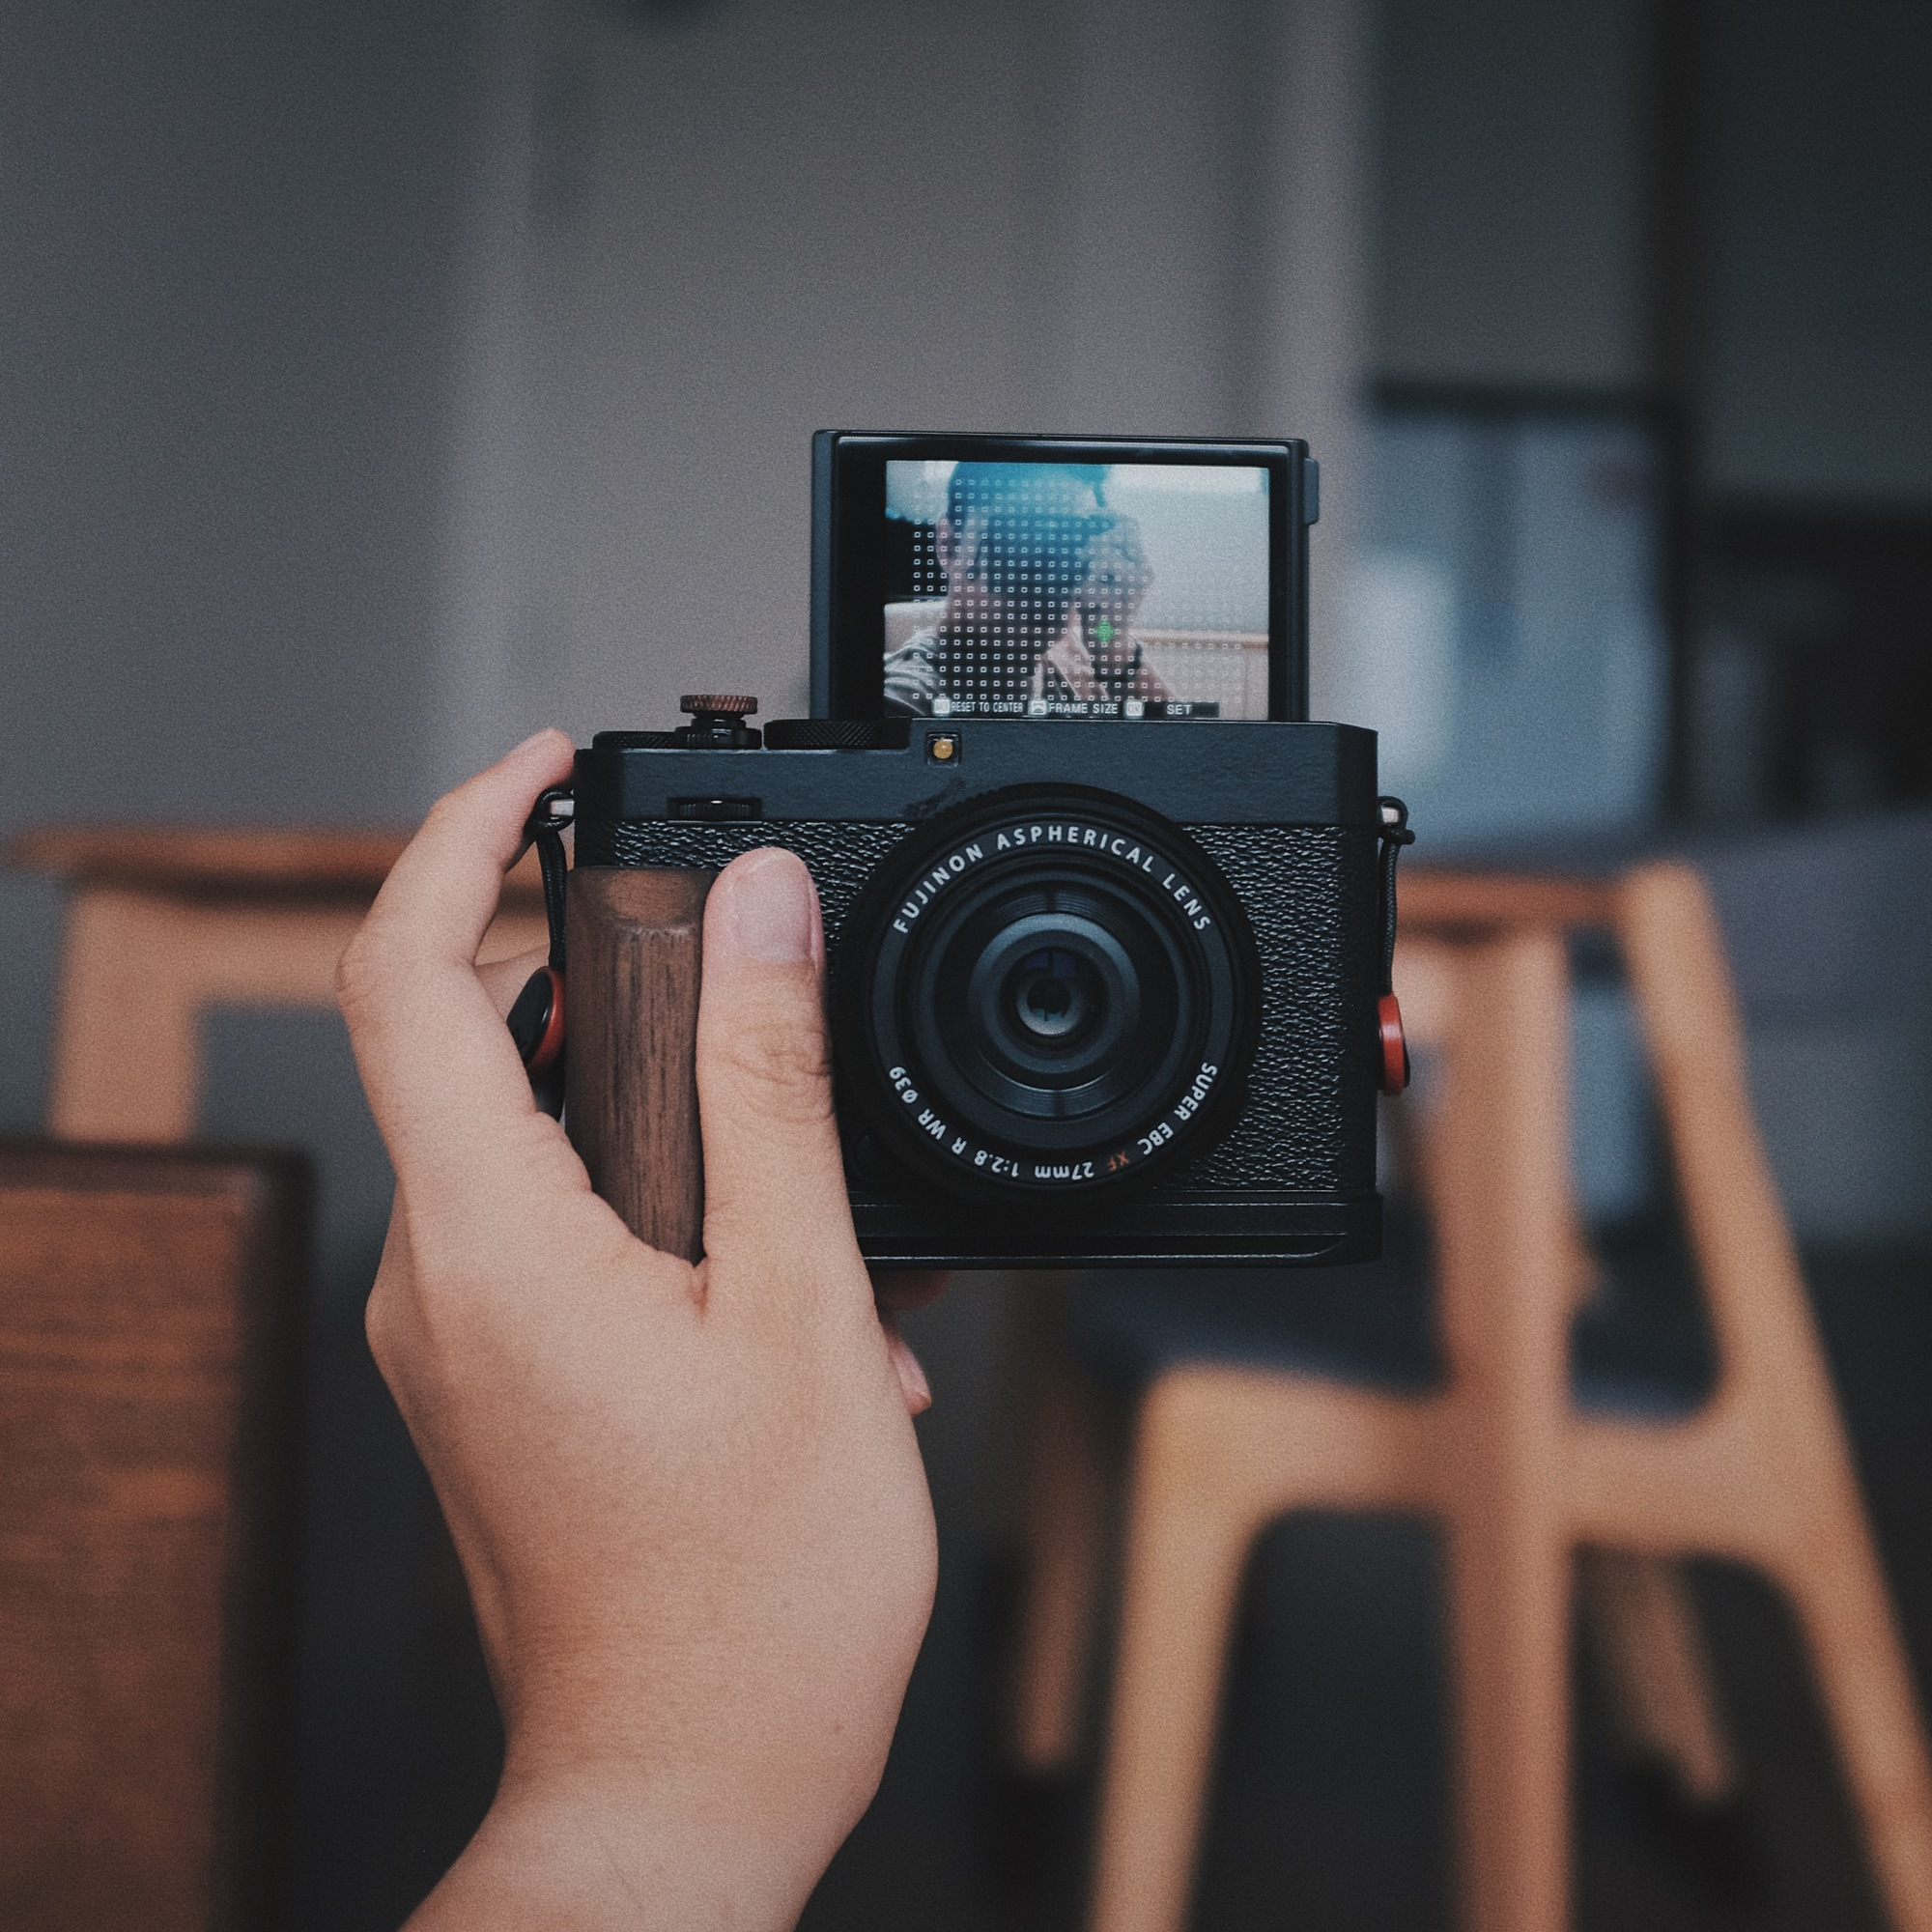
\includegraphics[width=\linewidth]{\envfinaldir/coverpic-prod.jpg}\par
            % \vskip 30pt
            \vfill

            \normalsize\rmfamily\scshape
            \copyright{} The Web Digest Project \hfill\large \envdatestr
        \end{center}
    \end{titlepage}
    % \restoregeometry
}
\newcommand{\simplehref}[1]{%
    \textcolor{blue!80!green}{\href{#1}{#1}}%
}
\renewcommand{\contentsname}{\center\Huge\sffamily\bfseries Contents\par\vskip 20pt}
\newcounter{ipartcounter}
\setcounter{ipartcounter}{0}
\newcommand{\ipart}[1]{
    % \vskip 20pt
    \clearpage
    \stepcounter{ipartcounter}
    \phantomsection
    \addcontentsline{toc}{chapter}{#1}
    % \begin{center}
    %     \Huge
    %     \sffamily\bfseries
    %     #1
    % \end{center}
    % \vskip 20pt plus 7pt
}
\newcounter{ichaptercounter}
\setcounter{ichaptercounter}{0}
\newcommand{\ichapter}[1]{
    % \vskip 20pt
    \clearpage
    \stepcounter{ichaptercounter}
    \phantomsection
    \addcontentsline{toc}{section}{\numberline{\arabic{ichaptercounter}}#1}
    \begin{center}
        \Huge
        \sffamily\bfseries
        #1
    \end{center}
    \vskip 20pt plus 7pt
}
\newcommand{\entrytitlefont}[1]{\subsection*{\raggedright\Large\sffamily\bfseries#1}}
\newcommand{\entryitemGeneric}[2]{
    % argv: title, url
    \parbox{\linewidth}{
        \entrytitlefont{#1}\par\vskip 5pt
        \footnotesize\ttfamily\mdseries
        \simplehref{#2}
    }\vskip 11pt plus 11pt minus 1pt
}
\newcommand{\entryitemGithub}[3]{
    % argv: title, url, desc
    \parbox{\linewidth}{
        \entrytitlefont{#1}\par\vskip 5pt
        \footnotesize\ttfamily\mdseries
        \simplehref{#2}\par\vskip 5pt
        \small\rmfamily\mdseries#3
    }\vskip 11pt plus 11pt minus 1pt
}
\newcommand{\entryitemAp}[3]{
    % argv: title, url, desc
    \parbox{\linewidth}{
        \entrytitlefont{#1}\par\vskip 5pt
        \footnotesize\ttfamily\mdseries
        \simplehref{#2}\par\vskip 5pt
        \small\rmfamily\mdseries#3
    }\vskip 11pt plus 11pt minus 1pt
}
\newcommand{\entryitemHackernews}[3]{
    % argv: title, hnurl, rawurl
    % \parbox{\linewidth}{
    %     \entrytitlefont{#1}\par\vskip 5pt
    %     \footnotesize\ttfamily\mdseries
    %     \simplehref{#3}\par
    %     \textcolor{black!50}{\href{#2}{#2}}
    % }\vskip 11pt plus 11pt minus 1pt
    \begin{minipage}{\linewidth}
            \entrytitlefont{#1}\par\vskip 5pt
            \footnotesize\ttfamily\mdseries
            \simplehref{#3}\par
            \textcolor{black!50}{\href{#2}{#2}}
    \end{minipage}\par\vskip 11pt plus 11pt minus 1pt
}







\begin{document}

\makeheader

\tableofcontents\clearpage




\ipart{Developers}
\ichapter{Hacker News}
\entryitemTwoLinks{FBI, EPA, and Treasury told Citibank to freeze funds to claw back climate money}{https://news.ycombinator.com/item?id=43366530}{https://techcrunch.com/2025/03/13/fbi-epa-and-treasury-told-citibank-to-freeze-funds-as-trump-administration-tries-to-claw-back-climate-money/}

\entryitemTwoLinks{Kerning, the Hard Way}{https://news.ycombinator.com/item?id=43366479}{https://home.octetfont.com/blog/kerning-hard.html}

\entryitemTwoLinks{Decrypting encrypted files from Akira ransomware using a bunch of GPUs}{https://news.ycombinator.com/item?id=43365083}{https://tinyhack.com/2025/03/13/decrypting-encrypted-files-from-akira-ransomware-linux-esxi-variant-2024-using-a-bunch-of-gpus/}

\entryitemTwoLinks{The School Car Pickup Line Is a National Embarrassment}{https://news.ycombinator.com/item?id=43364761}{https://collegetowns.substack.com/p/the-school-car-pickup-line-is-a-national}

\entryitemTwoLinks{Making Postgres scale}{https://news.ycombinator.com/item?id=43364668}{https://pgdog.dev/blog/you-can-make-postgres-scale}

\entryitemTwoLinks{Samsung Q990D unresponsive after 1020 firmware update}{https://news.ycombinator.com/item?id=43364016}{https://us.community.samsung.com/t5/Home-Theater/Samsung-Q990D-unresponsive-after-1020-firmware-update/td-p/3168571}

\entryitemTwoLinks{A 2FA app that tells you when you get `314159` (2024)}{https://news.ycombinator.com/item?id=43363918}{https://blog.jacobstechtavern.com/p/building-a-2fa-app-that-detects-patterns}

\entryitemTwoLinks{Block Diffusion: Interpolating between autoregressive and diffusion models}{https://news.ycombinator.com/item?id=43363247}{https://arxiv.org/abs/2503.09573}

\entryitemTwoLinks{I'm Peter Roberts, immigration attorney who does work for YC and startups. AMA}{https://news.ycombinator.com/item?id=43363056}{https://news.ycombinator.com/item?id=43363056}

\entryitemTwoLinks{Briar: Peer to Peer Encrypted Messaging}{https://news.ycombinator.com/item?id=43363031}{https://briarproject.org/how-it-works/}

\entryitemTwoLinks{Stoicism's appeal to the rich and powerful (2019)}{https://news.ycombinator.com/item?id=43363014}{https://www.exurbe.com/stoicisms-appeal-to-the-rich-and-powerful/}

\entryitemTwoLinks{A look at Firefox forks}{https://news.ycombinator.com/item?id=43361959}{https://lwn.net/Articles/1012453/}

\entryitemTwoLinks{In S3 simplicity is table stakes}{https://news.ycombinator.com/item?id=43361737}{https://www.allthingsdistributed.com/2025/03/in-s3-simplicity-is-table-stakes.html}

\entryitemTwoLinks{Migrating from AWS to a European Cloud – How We Cut Costs by 62\%}{https://news.ycombinator.com/item?id=43361366}{https://www.hopsworks.ai/post/migrating-from-aws-to-a-european-cloud-how-we-cut-costs-by-62}

\entryitemTwoLinks{Tesla Cybertruck deliveries on hold as trims are flying off 'bulletproof' truck}{https://news.ycombinator.com/item?id=43361038}{https://electrek.co/2025/03/13/tesla-cybertruck-deliveries-are-on-hold-as-trims-are-flying-off-the-bulletproof-truck/}

\entryitemTwoLinks{AMD's Strix Halo under the hood}{https://news.ycombinator.com/item?id=43360894}{https://chipsandcheese.com/p/amds-strix-halo-under-the-hood}

\entryitemTwoLinks{I-cant-believe-its-not-webusb: Hacking around lack of WebUSB support in Firefox}{https://news.ycombinator.com/item?id=43360642}{https://github.com/ArcaneNibble/i-cant-believe-its-not-webusb}

\entryitemTwoLinks{Ex-Facebook director's new book paints brutal image of Mark Zuckerberg}{https://news.ycombinator.com/item?id=43360024}{https://www.sfgate.com/tech/article/ex-facebook-director-book-brutal-image-zuckerberg-20220239.php}

\entryitemTwoLinks{TinyKVM: Fast sandbox that runs on top of Varnish}{https://news.ycombinator.com/item?id=43358980}{https://info.varnish-software.com/blog/tinykvm-the-fastest-sandbox}

\entryitemTwoLinks{The Church FAQ}{https://news.ycombinator.com/item?id=43358947}{https://whatever.scalzi.com/2025/03/13/the-church-faq/}\ichapter{Phoronix}
\entryitemGeneric{\hskip 0pt{}Radeon RX 9070 Fan Speed Reporting \& Other Last Minute AMD Changes For Linux 6.15}{https://www.phoronix.com/news/RX-9070-Fan-Speed-Linux-6.15}

\entryitemGeneric{\hskip 0pt{}Git 2.49 Released With Faster Packing, Rust Foreign Language Interface}{https://www.phoronix.com/news/Git-2.49-Released}

\entryitemGeneric{\hskip 0pt{}Mediatek DRM Driver Adding MT8365 "Genio 350" Support In Linux 6.15}{https://www.phoronix.com/news/Mediatek-MT8365-DRM-Linux-6.15}

\entryitemGeneric{\hskip 0pt{}GCC 15 Deprecates Support For The ESA/390 Architecture}{https://www.phoronix.com/news/GCC-Deprecates-ESA-390}

\entryitemGeneric{\hskip 0pt{}Arm Shows Off Great Performance Results For PGO \& BOLT With LLVM/Clang}{https://www.phoronix.com/news/Arm-Fast-PGO-BOLT-LLVM-Clang}

\entryitemGeneric{\hskip 0pt{}Glibc's Hyperbolic Functions Score Nice Speed-Ups With FMA Optimizations}{https://www.phoronix.com/news/glibc-Faster-Hyperbolic-FMA}

\entryitemGeneric{\hskip 0pt{}Mesa RADV/RadeonSI Now Support RDNA4 GPUs With Radeon GPU Profiler}{https://www.phoronix.com/news/Mesa-RDNA4-AMD-RGP}

\entryitemGeneric{\hskip 0pt{}Free95 0.2 Alpha Released As Open-Source Windows Compatible OS}{https://www.phoronix.com/news/Free95-0.2-Alpha}

\entryitemGeneric{\hskip 0pt{}IGT GPU Tools 2.0 Released For Helping To Develop DRM Drivers}{https://www.phoronix.com/news/IGT-GPU-Tools-2.0}\ichapter{Dribbble}
\entryitemGeneric{\hskip 0pt{}Triceratops}{https://dribbble.com/shots/25761010-Triceratops}

\entryitemGeneric{\hskip 0pt{}Tab Bar Animation}{https://dribbble.com/shots/25760227-Tab-Bar-Animation}

\entryitemGeneric{\hskip 0pt{}Chief Logo Design Process}{https://dribbble.com/shots/25759736-Chief-Logo-Design-Process}

\entryitemGeneric{\hskip 0pt{}World Clock App Design}{https://dribbble.com/shots/25760174-World-Clock-App-Design}

\entryitemGeneric{\hskip 0pt{}Carbon Solutions B2B Dashboard Design}{https://dribbble.com/shots/25681782-Carbon-Solutions-B2B-Dashboard-Design}

\entryitemGeneric{\hskip 0pt{}Logowave Awards Entry from Lepisov Branding}{https://dribbble.com/shots/25755190-Logowave-Awards-Entry-from-Lepisov-Branding}

\entryitemGeneric{\hskip 0pt{}Bir-D / D.Bird}{https://dribbble.com/shots/25757221-Bir-D-D-Bird}

\entryitemGeneric{\hskip 0pt{}Flare - Logo Design 🚀}{https://dribbble.com/shots/25754585-Flare-Logo-Design}

\entryitemGeneric{\hskip 0pt{}Squid Book}{https://dribbble.com/shots/25756273-Squid-Book}

\entryitemGeneric{\hskip 0pt{}Order detail dashboard}{https://dribbble.com/shots/25748173-Order-detail-dashboard}

\entryitemGeneric{\hskip 0pt{}Pricing Plan Web Page Design}{https://dribbble.com/shots/25755045-Pricing-Plan-Web-Page-Design}

\entryitemGeneric{\hskip 0pt{}Fishing Tournament Logo}{https://dribbble.com/shots/25750107-Fishing-Tournament-Logo}

\entryitemGeneric{\hskip 0pt{}Triceratops}{https://dribbble.com/shots/25749787-Triceratops}

\entryitemGeneric{\hskip 0pt{}Lamar® 21°}{https://dribbble.com/shots/25750164-Lamar-21}

\entryitemGeneric{\hskip 0pt{}Sergeant Scooper}{https://dribbble.com/shots/25749566-Sergeant-Scooper}

\entryitemGeneric{\hskip 0pt{}Atoms - Logo Concepts}{https://dribbble.com/shots/25749091-Atoms-Logo-Concepts}

\entryitemGeneric{\hskip 0pt{}Line Icons}{https://dribbble.com/shots/25749882-Line-Icons}

\entryitemGeneric{\hskip 0pt{}Logo For Designed.supply}{https://dribbble.com/shots/25748434-Logo-For-Designed-supply}

\entryitemGeneric{\hskip 0pt{}Logo Database (V7) 2024—25}{https://dribbble.com/shots/25743610-Logo-Database-V7-2024-25}

\entryitemGeneric{\hskip 0pt{}Codila Studio}{https://dribbble.com/shots/25749456-Codila-Studio}

\entryitemGeneric{\hskip 0pt{}Crystal // Website}{https://dribbble.com/shots/25742820-Crystal-Website}

\entryitemGeneric{\hskip 0pt{}Sway}{https://dribbble.com/shots/25744097-Sway}

\entryitemGeneric{\hskip 0pt{}Emergency App Concept Design}{https://dribbble.com/shots/25711688-Emergency-App-Concept-Design}

\entryitemGeneric{\hskip 0pt{}Partify}{https://dribbble.com/shots/25040893-Partify}


\ipart{Developers~~~~(zh-Hans)}
\ichapter{Solidot}
\entryitemGeneric{\hskip 0pt{}OpenAI 希望使用版权材料训练 AI 属于合理使用}{https://www.solidot.org/story?sid=80790}

\entryitemGeneric{\hskip 0pt{}澳大利亚男子在安装钛合金人造心脏后生存了 100 天}{https://www.solidot.org/story?sid=80789}

\entryitemGeneric{\hskip 0pt{}微软称 Windows 最近的一个更新会导致 USB 打印机打印随机文本}{https://www.solidot.org/story?sid=80788}

\entryitemGeneric{\hskip 0pt{}中生代哺乳动物有着深色皮毛}{https://www.solidot.org/story?sid=80787}

\entryitemGeneric{\hskip 0pt{}侏儒狐猴被发现会在冬眠时延长端粒}{https://www.solidot.org/story?sid=80786}

\entryitemGeneric{\hskip 0pt{}西欧发现已知最古老的人族脸部化石}{https://www.solidot.org/story?sid=80785}

\entryitemGeneric{\hskip 0pt{}微软试图统一 Windows 和 Xbox}{https://www.solidot.org/story?sid=80784}

\entryitemGeneric{\hskip 0pt{}Google 称 Gemma 3 使用一张 H100 GPU 就能获得与 DeepSeek R1 相当的性能}{https://www.solidot.org/story?sid=80783}

\entryitemGeneric{\hskip 0pt{}D-Wave 称其量子退火处理器相比超算具有``量子优越性''}{https://www.solidot.org/story?sid=80782}

\entryitemGeneric{\hskip 0pt{}雄章鱼给雌性注射镇静剂以防止被吃掉}{https://www.solidot.org/story?sid=80781}

\entryitemGeneric{\hskip 0pt{}棕矮星的质量极限}{https://www.solidot.org/story?sid=80780}

\entryitemGeneric{\hskip 0pt{}沙特投资基金以 36 亿美元收购 Pokemon Go}{https://www.solidot.org/story?sid=80779}

\entryitemGeneric{\hskip 0pt{}英特尔任命陈立武为新 CEO }{https://www.solidot.org/story?sid=80778}

\entryitemGeneric{\hskip 0pt{}全球智能手表销量首次下滑}{https://www.solidot.org/story?sid=80777}

\entryitemGeneric{\hskip 0pt{}iRobot 警告它可能在 12 个月内倒闭}{https://www.solidot.org/story?sid=80776}

\entryitemGeneric{\hskip 0pt{}长时间玩游戏对幸福感影响不大}{https://www.solidot.org/story?sid=80775}

\entryitemGeneric{\hskip 0pt{}微软用 Windows App 替代 Remote Desktop app}{https://www.solidot.org/story?sid=80774}

\entryitemGeneric{\hskip 0pt{}至少 1.1 \% 的中世纪手稿是修女抄写的}{https://www.solidot.org/story?sid=80773}

\entryitemGeneric{\hskip 0pt{}Spotify 在 2024 年支付了 100 亿美元版税}{https://www.solidot.org/story?sid=80772}

\entryitemGeneric{\hskip 0pt{}Meta 开始测试其自研 AI 训练芯片}{https://www.solidot.org/story?sid=80771}\ichapter{V2EX}
\entryitemGeneric{\hskip 0pt{}[OpenWrt] Openwrt x86 内核 6.6.79,分支: 24.10,挺多 bug 的}{https://www.v2ex.com/t/1118578}

\entryitemGeneric{\hskip 0pt{}[Apple] 有什么办法让 mac 保留``镜像或拓展至 iPad ''吗}{https://www.v2ex.com/t/1118577}

\entryitemGeneric{\hskip 0pt{}[创业组队] 一个找聊天搭子的社交产品创意。}{https://www.v2ex.com/t/1118576}

\entryitemGeneric{\hskip 0pt{}[汽车] 开车出去游山玩水的,中顶轻卡(2.0m-2.2m)想下停车场地库 基本上都可以的吧?}{https://www.v2ex.com/t/1118575}

\entryitemGeneric{\hskip 0pt{}[站长] 网页增加亮暗主题切换按钮的方式}{https://www.v2ex.com/t/1118574}

\entryitemGeneric{\hskip 0pt{}[浏览器] chrome 插件强制 mv3 标准之后广告拦截插件都不能自定义规则了, 但 safari 可以}{https://www.v2ex.com/t/1118573}

\entryitemGeneric{\hskip 0pt{}[iOS] 这辈子都没见过的奇特 iOS bug}{https://www.v2ex.com/t/1118572}

\entryitemGeneric{\hskip 0pt{}[汽车] 准备买车,基本在路上玩的 半床车吧, 玩累了就车床上,单人就凑合下}{https://www.v2ex.com/t/1118571}

\entryitemGeneric{\hskip 0pt{}[分享发现] 最近几个月需要开车上班,每天都听牛人的访谈给自己打气}{https://www.v2ex.com/t/1118570}

\entryitemGeneric{\hskip 0pt{}[推广] Gemma 3 Online(Free to use)}{https://www.v2ex.com/t/1118569}

\entryitemGeneric{\hskip 0pt{}[程序员] google 的新模型,智能文字修图,效果实在是很炸裂。}{https://www.v2ex.com/t/1118568}

\entryitemGeneric{\hskip 0pt{}[职场话题] 被公司要求延长一个月试用期}{https://www.v2ex.com/t/1118566}

\entryitemGeneric{\hskip 0pt{}[德国] 有在汉堡的 V 友吗?出来面基聊个天?}{https://www.v2ex.com/t/1118565}

\entryitemGeneric{\hskip 0pt{}[Apple] 想换苹果 MacBook Air M4 的冲动}{https://www.v2ex.com/t/1118564}

\entryitemGeneric{\hskip 0pt{}[Apple] 疯狂长草,如何购买 mac studio M4 MAX 丐版最划算?}{https://www.v2ex.com/t/1118563}

\entryitemGeneric{\hskip 0pt{}[问与答] 我的硬盘右正解动不动就弹窗,就是插入硬盘那种弹窗,}{https://www.v2ex.com/t/1118562}

\entryitemGeneric{\hskip 0pt{}[Android] 纠结要不要继续坚持国际版小米}{https://www.v2ex.com/t/1118561}

\entryitemGeneric{\hskip 0pt{}[问与答] Google Play 上架迟迟没有结果,``已签名的通用 APK''是否和 Play 版本签名一致}{https://www.v2ex.com/t/1118559}

\entryitemGeneric{\hskip 0pt{}[职场话题] 现在二线城市开发到底啥行情}{https://www.v2ex.com/t/1118558}

\entryitemGeneric{\hskip 0pt{}[Apple] 求助!苹果开发者账号被盗了,损失 100 多万, 2 个月了苹果没有回复...}{https://www.v2ex.com/t/1118557}

\entryitemGeneric{\hskip 0pt{}[程序员] 请教一下视频录制的右下角显示演讲者,是用的什么软件呢?想用}{https://www.v2ex.com/t/1118556}

\entryitemGeneric{\hskip 0pt{}[程序员] 请教老师们,类似百度地图 API 并发峰值上限约束不能超过 100/秒,程序上是不是没法精确控制?(我主要用来获取地图经纬度,我用 Claude 3.7 Sonnet 帮忙写的,似乎无法精确控制)}{https://www.v2ex.com/t/1118555}

\entryitemGeneric{\hskip 0pt{}[YouTube] YoTube 突然画质变差}{https://www.v2ex.com/t/1118554}

\entryitemGeneric{\hskip 0pt{}[程序员] 关于 windows11 蓝牙突然没了?只能自己重新下载驱动才可以?}{https://www.v2ex.com/t/1118553}

\entryitemGeneric{\hskip 0pt{}[职场话题] AI 行业就业岗位分析?通过分析各个公司的的人才储备情况来判断当前市场的趋势?}{https://www.v2ex.com/t/1118552}

\entryitemGeneric{\hskip 0pt{}[C++] C++库脚手架项目及思考}{https://www.v2ex.com/t/1118551}

\entryitemGeneric{\hskip 0pt{}[问与答] 有人玩星际重制版吗?}{https://www.v2ex.com/t/1118550}

\entryitemGeneric{\hskip 0pt{}[Android] 关于国内安卓系的广告}{https://www.v2ex.com/t/1118549}

\entryitemGeneric{\hskip 0pt{}[OpenWrt] mosdns 如何使用 ipv6 的 DNS 服务器?}{https://www.v2ex.com/t/1118548}

\entryitemGeneric{\hskip 0pt{}[问与答] 有尺度比较大的开源 ai 大模型吗?}{https://www.v2ex.com/t/1118547}

\entryitemGeneric{\hskip 0pt{}[搜索引擎优化] 挑战一下, 30 天新站 DR 过 40}{https://www.v2ex.com/t/1118545}

\entryitemGeneric{\hskip 0pt{}[推广] 顶级域名 CV 正在开放注册,附优质域名 50\%折扣码}{https://www.v2ex.com/t/1118544}

\entryitemGeneric{\hskip 0pt{}[酷工作] iOS/Andriod 开发\_初创项目\_可 Remote\_可兼职}{https://www.v2ex.com/t/1118543}

\entryitemGeneric{\hskip 0pt{}[Windows] 求助求助, Dell 迷你机的 intel 核显上不了 2K 分辨率}{https://www.v2ex.com/t/1118542}

\entryitemGeneric{\hskip 0pt{}[商业模式] 19 岁香港留学生,将临期面包变新品,年入百万}{https://www.v2ex.com/t/1118540}

\entryitemGeneric{\hskip 0pt{}[酷工作] 社招内推:资深大数据开发工程师\_传音控股}{https://www.v2ex.com/t/1118538}

\entryitemGeneric{\hskip 0pt{}[问与答] 有没有人能做一个 AI 标识去除器,绝对大火}{https://www.v2ex.com/t/1118537}

\entryitemGeneric{\hskip 0pt{}[全球工单系统] 用移动 APP 充值话费,被微信限制支付了,提示是涉嫌赌博,是移动的问题,还是微信支付的问题?}{https://www.v2ex.com/t/1118536}

\entryitemGeneric{\hskip 0pt{}[程序员] 为什么 il2cpp、Nuitka 等把其它语言编译成机器码都需要使用 C++作为中间语言编译两次,.NET 8 的 AOT 可以一步到位?中间语言为什么是 C++,不是 C、更安全的 Rust?}{https://www.v2ex.com/t/1118535}

\entryitemGeneric{\hskip 0pt{}[酷工作] [上海] 米哈游预研项目火热招聘中~~2025.3.14}{https://www.v2ex.com/t/1118534}

\entryitemGeneric{\hskip 0pt{}[程序员] 相亲经历}{https://www.v2ex.com/t/1118533}

\entryitemGeneric{\hskip 0pt{}[酷工作] 校招内推: AI 算法、AI 产品、后端、Android、运维、测试等\_传音控股 2025 届春招全面启动}{https://www.v2ex.com/t/1118532}

\entryitemGeneric{\hskip 0pt{}[问与答] 打游戏时电脑出现没规律短时断网}{https://www.v2ex.com/t/1118531}

\entryitemGeneric{\hskip 0pt{}[问与答] 虚拟机安装游戏}{https://www.v2ex.com/t/1118530}

\entryitemGeneric{\hskip 0pt{}[Python] 如何在 jupyter notebook 里安装 binance 模块?有没有会 Python 的大神来指点下?}{https://www.v2ex.com/t/1118529}

\entryitemGeneric{\hskip 0pt{}[路由器] 华硕小旋风 be3600 be6500 出官改固件了}{https://www.v2ex.com/t/1118528}

\entryitemGeneric{\hskip 0pt{}[问与答] 求推荐一个聚合支付支持分润}{https://www.v2ex.com/t/1118527}

\entryitemGeneric{\hskip 0pt{}[问与答] 在西安办理那个宽带最划算}{https://www.v2ex.com/t/1118526}

\entryitemGeneric{\hskip 0pt{}[程序员] 怎么从浏览器打开飞书, 并跳到与指定工号人员的聊天框, 并携带订单号}{https://www.v2ex.com/t/1118525}

\entryitemGeneric{\hskip 0pt{}[求职] 7 年前端大厂背景,求职最好是 web3 或者可以 remote 的}{https://www.v2ex.com/t/1118524}


\ipart{Generic News}







\clearpage
\leavevmode\vfill
\footnotesize

Copyright \copyright{} 2023-2025 Neruthes and other contributors.

This document is published with CC BY-NC-ND 4.0 license.

The entries listed in this newsletter may be copyrighted by their respective creators.

This newsletter is generated by the Web Digest project.

The newsletters are also delivered via Telegram channel \CJKunderline{\href{https://t.me/webdigestchannel}{https://t.me/webdigestchannel}}.\\
RSS feed is available at \CJKunderline{\href{https://webdigest.pages.dev/rss.xml}{https://webdigest.pages.dev/rss.xml}}.

This newsletter is available in PDF at
\CJKunderline{\href{https://webdigest.pages.dev/}{https://webdigest.pages.dev/}}.

The source code being used to generate this newsletter is available at\\
\CJKunderline{\href{https://github.com/neruthes/webdigest}{https://github.com/neruthes/webdigest}}.

This newsletter is also available in
\CJKunderline{\href{http://webdigest.pages.dev/readhtml/\envyear/WebDigest-20250315.html}{HTML}} and
\CJKunderline{\href{https://github.com/neruthes/webdigest/blob/master/markdown/\envyear/WebDigest-20250315.md}{Markdown}}.


\coverpic{https://unsplash.com/photos/a-house-in-the-middle-of-a-snowy-field-zMxhdWSnSiY}{Philipp Düsel}


\end{document}
